\documentclass[border=10pt,tikz]{standalone}
\usepackage{tikz}
\usetikzlibrary{positioning,arrows.meta,shapes,backgrounds,fit}

\begin{document}
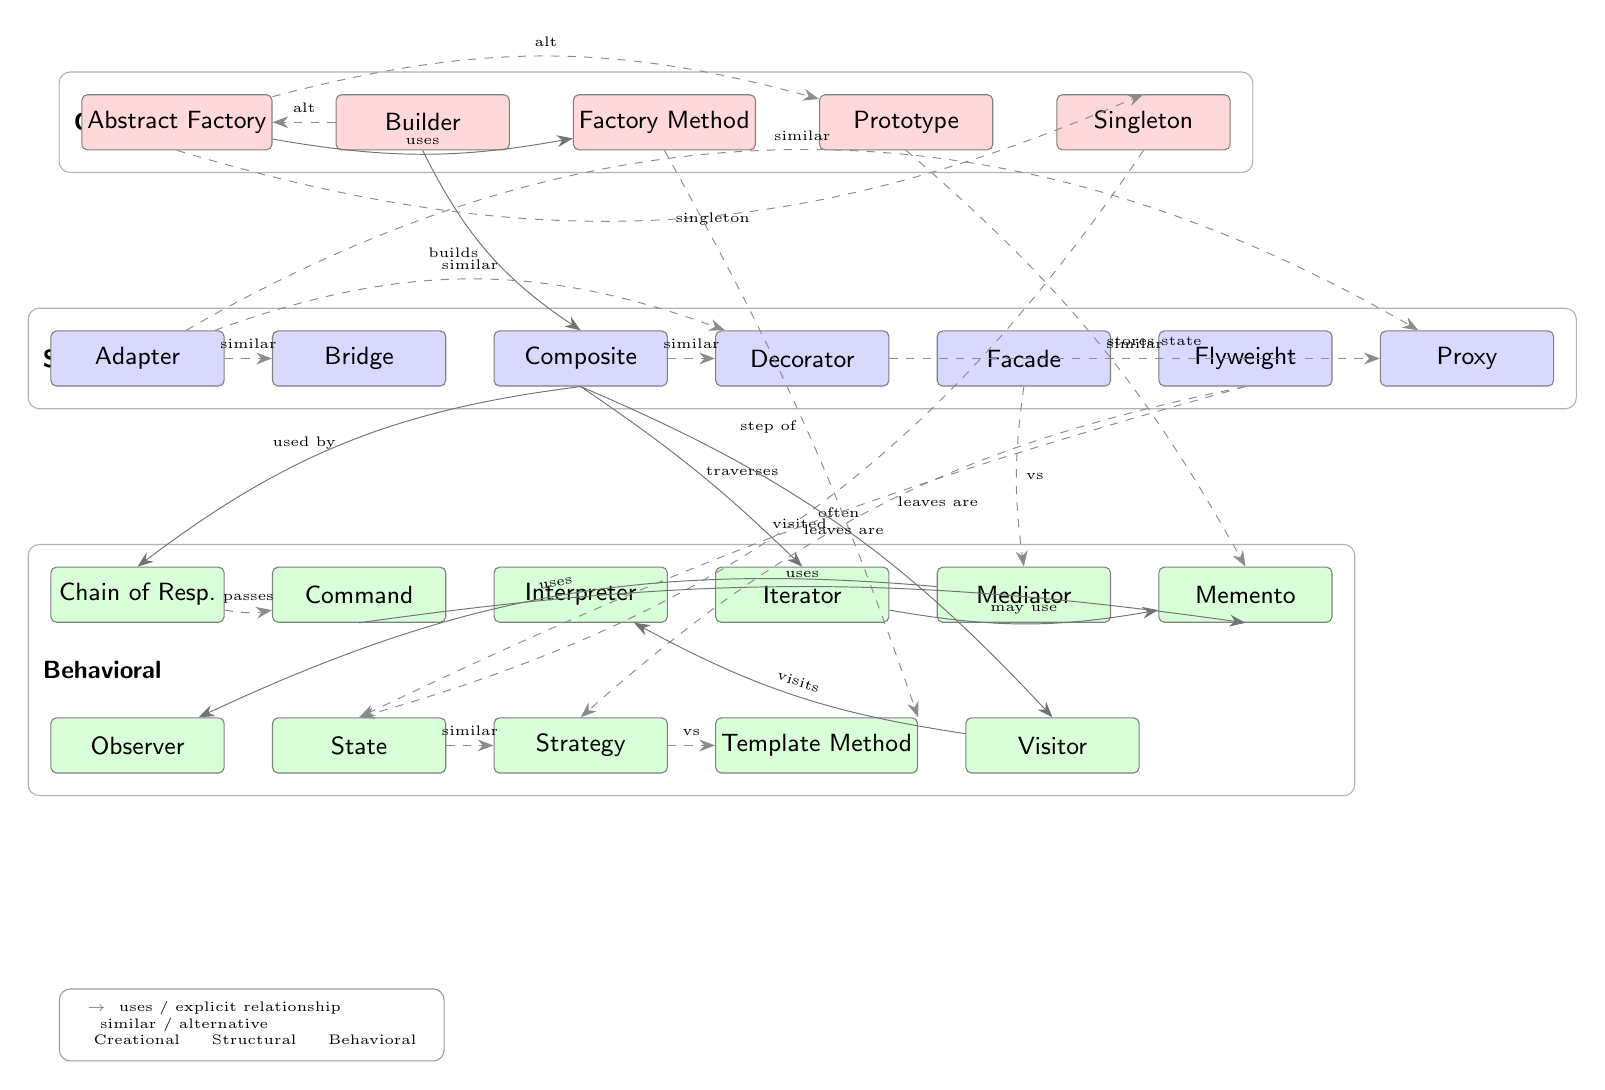
\begin{tikzpicture}[
  font=\sffamily\small,
  pattern/.style={
    rectangle, rounded corners=2pt,
    draw=black!50, line width=0.4pt,
    minimum height=7mm, minimum width=22mm,
    inner sep=2pt, fill=white
  },
  creational/.style={pattern, fill=red!15},
  structural/.style={pattern, fill=blue!15},
  behavioral/.style={pattern, fill=green!15},
  rel/.style={->, >={Stealth[length=2mm]}, draw=black!55, line width=0.35pt},
  reldash/.style={rel, dashed, draw=black!45},
  group/.style={rectangle, rounded corners, draw=black!30, line width=0.4pt, inner sep=8pt}
]

% ─── CREATIONAL (top) ───────────────────────────────────────────
\node[creational]                            (af)  at (-6, 5.5) {Abstract Factory};
\node[creational, right=8mm of af]           (bld) {Builder};
\node[creational, right=8mm of bld]          (fm)  {Factory Method};
\node[creational, right=8mm of fm]           (pt)  {Prototype};
\node[creational, right=8mm of pt]           (sg)  {Singleton};

\begin{scope}[on background layer]
\node[group, fit=(af)(bld)(fm)(pt)(sg), label={[anchor=west,xshift=2pt]left:\textbf{Creational}}] {};
\end{scope}

% ─── STRUCTURAL (middle) ────────────────────────────────────────
\node[structural]                            (adp) at (-6.5, 2.5) {Adapter};
\node[structural, right=6mm of adp]          (brd) {Bridge};
\node[structural, right=6mm of brd]          (cmp) {Composite};
\node[structural, right=6mm of cmp]          (dec) {Decorator};
\node[structural, right=6mm of dec]          (fcd) {Facade};
\node[structural, right=6mm of fcd]          (fly) {Flyweight};
\node[structural, right=6mm of fly]          (prx) {Proxy};

\begin{scope}[on background layer]
\node[group, fit=(adp)(brd)(cmp)(dec)(fcd)(fly)(prx), label={[anchor=west,xshift=2pt]left:\textbf{Structural}}] {};
\end{scope}

% ─── BEHAVIORAL (bottom, 2 rows) ────────────────────────────────
\node[behavioral]                            (cor) at (-6.5, -0.5) {Chain of Resp.};
\node[behavioral, right=6mm of cor]          (cmd) {Command};
\node[behavioral, right=6mm of cmd]          (intr){Interpreter};
\node[behavioral, right=6mm of intr]         (itr) {Iterator};
\node[behavioral, right=6mm of itr]          (med) {Mediator};
\node[behavioral, right=6mm of med]          (mem) {Memento};

\node[behavioral, below=12mm of cor]         (obs) {Observer};
\node[behavioral, right=6mm of obs]          (st)  {State};
\node[behavioral, right=6mm of st]           (str) {Strategy};
\node[behavioral, right=6mm of str]          (tm)  {Template Method};
\node[behavioral, right=6mm of tm]           (vis) {Visitor};

\begin{scope}[on background layer]
\node[group, fit=(cor)(cmd)(intr)(itr)(med)(mem)(obs)(st)(str)(tm)(vis), label={[anchor=west,xshift=2pt]left:\textbf{Behavioral}}] {};
\end{scope}

% ─── RELATIONSHIPS ──────────────────────────────────────────────
% Creational internal
\draw[rel] (af)  to[bend right=10] node[above,sloped,font=\tiny]{uses} (fm);
\draw[reldash] (af) to[bend left=15] node[above,sloped,font=\tiny]{alt} (pt);
\draw[reldash] (af.south) to[bend right=20] node[right,font=\tiny]{singleton} (sg.north);

% Builder relationships
\draw[reldash] (bld) -- node[above,sloped,font=\tiny]{alt} (af);

% Creational → Structural / Behavioral
\draw[rel] (bld.south) to[bend right=15] node[left,font=\tiny]{builds} (cmp.north);
\draw[reldash] (pt.south) to[bend left=10] node[right,font=\tiny]{stores state} (mem.north);
\draw[reldash] (sg.south) to[bend left=20] node[right,font=\tiny]{often} (st.north);
\draw[reldash] (fm.south) to[bend left=5]  node[left,font=\tiny]{step of} (tm.north east);

% Structural internal
\draw[reldash] (adp) -- node[above,font=\tiny]{similar} (brd);
\draw[reldash] (adp) to[bend left=20] node[above,font=\tiny]{similar} (dec);
\draw[reldash] (adp) to[bend left=30] node[above,font=\tiny]{similar} (prx);
\draw[reldash] (dec) -- node[above,font=\tiny]{similar} (prx);
\draw[reldash] (cmp) -- node[above,font=\tiny]{similar} (dec);

% Structural → Behavioral
\draw[rel] (cmp.south) to[bend left=5] node[right,font=\tiny]{traverses} (itr.north);
\draw[rel] (cmp.south) to[bend left=12] node[left,font=\tiny]{visited} (vis.north);
\draw[rel] (cmp.south) to[bend right=15] node[left,font=\tiny]{used by} (cor.north);
\draw[reldash] (fly.south) to[bend right=5] node[right,font=\tiny]{leaves are} (st.north);
\draw[reldash] (fly.south) to[bend right=15] node[right,font=\tiny]{leaves are} (str.north);
\draw[reldash] (fcd.south) to[bend right=8] node[right,font=\tiny]{vs} (med.north);

% Behavioral internal
\draw[reldash] (cor) to[bend right=10] node[above,font=\tiny]{passes} (cmd);
\draw[rel] (cmd.south) to[bend left=8] node[above,sloped,font=\tiny]{uses} (mem.south);
\draw[reldash] (st) -- node[above,font=\tiny]{similar} (str);
\draw[reldash] (str) -- node[above,font=\tiny]{vs} (tm);
\draw[rel] (med) to[bend right=15] node[above,sloped,font=\tiny]{uses} (obs);
\draw[rel] (vis) to[bend left=10] node[above,sloped,font=\tiny]{visits} (intr);
\draw[rel] (itr) to[bend right=10] node[above,sloped,font=\tiny]{may use} (mem);

% Legend
\node[draw=black!40, rounded corners, inner sep=4pt, font=\tiny, anchor=north west]
  at (-7.5, -5.5) {\begin{tabular}{l}
    \textcolor{black!55}{$\rightarrow$} \ uses / explicit relationship \\
    \textcolor{black!45}{$\dashrightarrow$} \ similar / alternative \\
    \textcolor{red!15!black}{$\blacksquare$} Creational \quad
    \textcolor{blue!15!black}{$\blacksquare$} Structural \quad
    \textcolor{green!30!black}{$\blacksquare$} Behavioral
  \end{tabular}};

\end{tikzpicture}
\end{document}
